\documentclass[10pt]{article}
\usepackage[utf8]{inputenc}
\usepackage[T1]{fontenc}
\usepackage{amsmath,amssymb}
\newcommand{\numberset}{\mathbb}
\usepackage{mathptmx}
\usepackage[italian]{babel}
\usepackage{newlfont}
\usepackage{color}
\textwidth=450pt\oddsidemargin=0pt
\usepackage{textcomp}
\usepackage{amsfonts}
\usepackage{amsthm}
\usepackage{braket}
\usepackage{bbold}
\usepackage[margin=2.8cm]{geometry}
\usepackage{fancyhdr}
\usepackage{systeme,mathtools}
\usepackage{float}
\usepackage{relsize}
\usepackage{dsfont}
\usepackage{calligra}
\usepackage{hyperref}
\usepackage{circuitikz}
\usepackage{epstopdf}
\usepackage{float}
\usepackage{listings}
\usepackage{titling}
\usepackage{graphicx}
\graphicspath{{./images/}}
\usepackage[table,xcdraw]{xcolor}

\begin{document}

\begin{titlepage}
  \begin{center}
  {{\Large{\textsc{Università degli Studi di Urbino Carlo Bo}}}} 
  \\\vspace{2mm}
  
  {\normalsize{\bf Corso di Laurea in Informatica Applicata}}
  \end{center}
  
      \vspace{40mm}
      \begin{center}
      {\Large\bf{Prodotto di differenze di valori a 4 bit}} 
      \end{center}
      
      \vspace{10mm}
      
      \begin{center}
      {\Large{Progetto d'esame di Reti Logiche 
      \vspace{3mm}}}
      \end{center}
      
      \vspace{10mm}
      
      \begin{center}
      {\Large A.A 2022/23 
      \vspace{3mm}}
      \end{center}
      
      \vspace{80mm} \par \noindent
      
  \begin{minipage}[t]{0.35\textwidth}
  %
  {\large Balducci Milena}
  \end{minipage}
  %
  \hfill
  %
  \begin{minipage}[t]{0.35\textwidth}\raggedleft \textcolor{black}{
  {\large Matricola 321791}}
  \end{minipage}
  \end{titlepage}

\newpage

\section{Specifica}

\subsection{Scopo del progetto}
L'obiettivo è quello di realizzare una rete combinatoria in tecnologia CMOS dotata di quattro ingressi A e B a 4 bit, rappresentanti quattro valori in codifica binaria naturale, 
e di una uscita Z a 8 bit che rappresenta il prodotto delle differenze dei quattro valori in ingresso.

\subsection{Specifica funzionale}
$f:{\mathbb{N}^4} \longrightarrow \mathbb{N}, \ \ f(a,b,c,d) = (a-b)\cdot (c-d)$.
\newpage

\section{Impostazione progetto a livello RT}

\subsection{Data Flow Graph}
$f = (a-b) * (a-b)$
\begin{figure}[H]
    \centering
    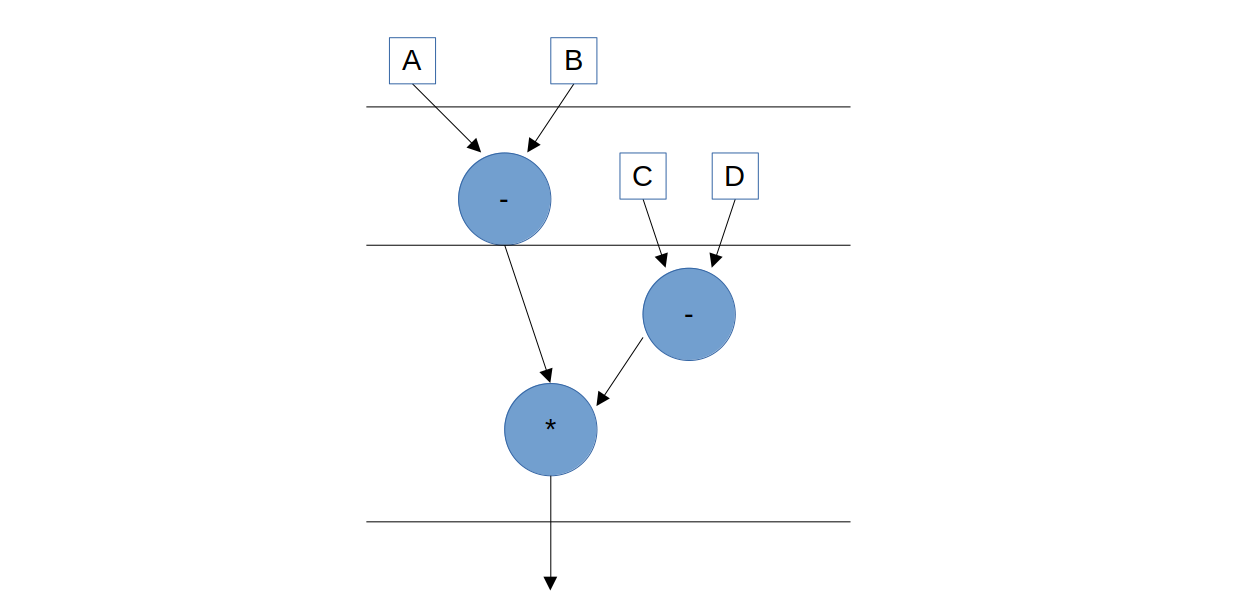
\includegraphics[width=0.8\textwidth]{dfg}
\end{figure}

Dal momento che l'operazione di sottrazione compare due volte all'interno del data flow graph, è possibile utilizzare il resource sharing, usando una unica macro aritmetica per entrambe le differenze.
Per fare questo sono necessari due cicli di clocK: durante il primo viene svolta la differenza tra i primi due valori, e durante il secondo viene svolta la seconda differenza e il prodotto tra i due
risultati. 
Per svolgere la differenza tra due numeri si è scelto di utilizzare la notifica in complemento a due, il secondo valore andrà dunque convertito nel rispettivo complemento prima di essere passato
ad un addizionatore.

\subsection{Risorse}
    \begin{itemize}
        \item 3 Registri a 4 bit
        \item 2 Multiplexer a 2 ingressi a 4 bit
        \item 1 Demultiplexer a 2 uscite a 4 bit
        \item 1 Complementatore a 4 bit
        \item 1 Addizionatore a 4 bit
        \item 1 Moltiplicatore a ingressi a 4 bit e uscita a 8 bit
    \end{itemize}
\newpage

\section{Progetto delle risorse a livello gate}
Per progettare i componenti necessari alla realizzazione della rete combinatoria illustrata nella specifica, è necessario
partire dalle porte logiche. Queste vengono realizzate partendo dai due componenti base della tecnologia C-MOS: i transistor \textbf{nMOS} e \textbf{pMOS}.
Questi due transistor sono formati da tre terminali: \textbf{Source (S)}, \textbf{Drain (D)} e \textbf{Gate (G)}.

\begin{figure}[H]
    \centering
    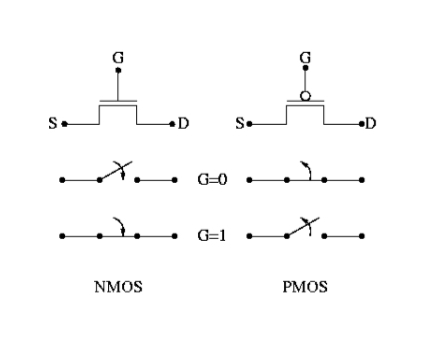
\includegraphics[width=0.8\textwidth]{transistors}    
\end{figure}

\begin{itemize}
    \item Il transistor \textbf{nMOS} crea un collegamento tra S e D solo se il Gate assume valore 1 (alto).
    Quando viene collegato a massa, si forma la rete di \textbf{"pull-down"}.
    \item Il transistor \textbf{pMOS} collega S e D solo se il valore del Gate è 0 (basso). Quando collegato alla Vdd,
    forma quella che si chiama rete di \textbf{"pull-up"}.

\subsection{Porte logiche semplici}
Le porte logiche elementari sono quelle corrispondenti agli operatori logici di base, a partire dai quali è possibile costruire tutti gli altri operatori (e, di conseguenza, le altre
porte logiche). Queste sono le porte \textbf{NOT}, \textbf{NAND} e \textbf{NOR}. Tutte le porte logiche possono avere un numero arbitratio di ingressi. 
Tuttavia, in questo progetto si è fatto uso esclusivamente di porte a due ingressi, quindi da qui in avanti le descrizioni e le tabelle della verità faranno riferimento a questo tipo di porte logiche.

\subsubsection{Porta NOT}
La porta NOT (o inverter), corrispondente all'omonimo operatore logico, prende il segnale in ingresso e lo restituisce negato. Viene realizzata collegando in serie pull-up e pull-down. Di seguito 
sono illustrate la tabella della verità e l'implementazione della porta NOT.
\begin{table}[ht]
    \begin{minipage}[b]{0.4\textwidth}
    \centering
    \begin{tabular}{ | l | l |}
        \hline
           X    &    X'   \\ \hline	
           0    &    1    \\ 
           1    &    0    \\ \hline
       \end{tabular}
        \caption{Tabella della verità inverter}
        \label{table:student}
    \end{minipage}
    \end{table}
    
    \begin{figure}[ht]
    \begin{minipage}[b]{0.4\textwidth}
    
    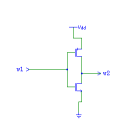
\includegraphics[width=70mm]{inverter}
    \caption{Implementazione inverter}
    \label{ }
    \end{minipage}
    \end{figure}


\subsubsection{Porta NAND}
La porta NAND è una porta logica invertente che restituisce 1 solo se almeno uno dei due ingressi vale 0, e corrisponde alla negazione della congiunzione logica dei due ingressi. 
Si tratta di una porta logica semplice in quanto è funzionalmente completa, ovvero a partire da essa è possibile implementare tutte le altre porte logiche. 
Viene realizzata collegando in parallelo due transistor pMOS e in serie due transistor nMOS.

\begin{table}[H]
    \begin{minipage}[b]{0.4\textwidth}
    \centering
    \begin{tabular}{|ll|l|}
    \hline
    \textbf{A} & \textbf{B} & \textbf{Y} \\ \hline
    0          & 0          & 1          \\ 
    0          & 1          & 1          \\ 
    1          & 0          & 1          \\ 
    1          & 1          & 0          \\ \hline
    \end{tabular}
        \caption{Tabella della verità NAND}
        \label{table:student}
    \end{minipage}
    \end{table}
    
    \begin{figure}[ht]
    \begin{minipage}[b]{0.4\textwidth}
    
    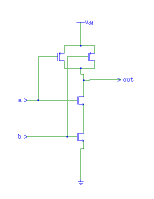
\includegraphics[width=70mm]{nand}
    \caption{Implementazione NAND}
    \label{ }
    \end{minipage}
    \end{figure}

\subsubsection{Porta NOR}
La porta NOR è una porta logica invertente che restituisce 1 solo se entrambi gli ingressi valgono 0, e corrisponde alla negazione della disgiunzione logica dei due ingressi. 
Come per il NAND, questa porta è funzionalmente completa. 
Viene realizzata collegando in parallelo due transistor nMOS e in serie due transistor pMOS.

\begin{table}[H]
    \begin{minipage}[b]{0.4\textwidth}
    \centering
    \begin{tabular}{|ll|l|}
    \hline
    \textbf{A} & \textbf{B} & \textbf{Y} \\ \hline
    0          & 0          & 1          \\ 
    0          & 1          & 0          \\ 
    1          & 0          & 0          \\ 
    1          & 1          & 0          \\ \hline
    \end{tabular}
        \caption{Tabella della verità NOR}
        \label{table:student}
    \end{minipage}
    \end{table}
    
    \begin{figure}[ht]
    \begin{minipage}[b]{0.4\textwidth}
    
    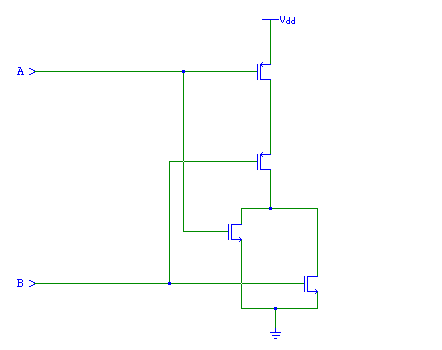
\includegraphics[width=70mm]{nor}
    \caption{Implementazione NOR}
    \label{ }
    \end{minipage}
    \end{figure}

\subsection{Porte logiche composte}
Le porte logiche composte utilizzate in questo progetto sono le porte AND, OR e EXOR. Ciascuna di queste è realizzata combinando porte NOT, NAND e NOR.

\subsubsection{Porta AND}
La porta AND è realizzata tramite una porta NAND, la cui uscita viene invertita tramite una porta NOT.
\begin{table}[H]
    \begin{minipage}[b]{0.4\textwidth}
    \centering
    \begin{tabular}{|ll|l|}
        \hline
        \textbf{A} & \textbf{B} & \textbf{((AB)')' = AB} \\ \hline
        0          & 0          & 0          \\ \hline
        0          & 1          & 0          \\ 
        1          & 0          & 0          \\ 
        1          & 1          & 1          \\ \hline
        \end{tabular}
        \caption{Tabella della verità AND}
        \label{table:student}
    \end{minipage}
    \end{table}
    
    \begin{figure}[ht]
    \begin{minipage}[b]{0.4\textwidth}
    
    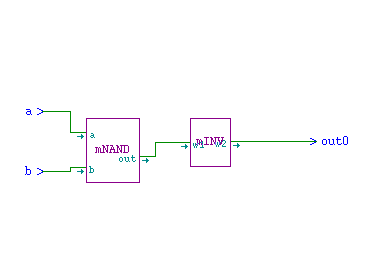
\includegraphics[width=70mm]{and}
    \caption{Implementazione NAND}
    \label{ }
    \end{minipage}
    \end{figure}

\subsubsection{Porta OR}
E' possibile realizzare una porta OR, che corrisponde all'omonimo operatore logico, semplicemente invertendo l'uscita di una porta NOR.

    \begin{table}[H]
        \begin{minipage}[b]{0.4\textwidth}
        \centering
        \begin{tabular}{|ll|l|}
            \hline
            \textbf{A} & \textbf{B} & \textbf{((A+B)')' = A + B} \\ \hline
            0          & 0          & 0          \\ \hline
            0          & 1          & 1          \\ 
            1          & 0          & 1          \\ 
            1          & 1          & 1          \\ \hline
            \end{tabular}
            \caption{Tabella della verità OR}
            \label{table:student}
        \end{minipage}
        \end{table}
        
        \begin{figure}[ht]
        \begin{minipage}[b]{0.4\textwidth}
        
        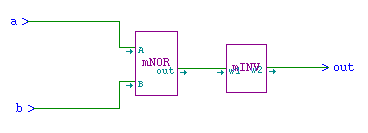
\includegraphics[width=70mm]{or}
        \caption{Implementazione OR}
        \label{ }
        \end{minipage}
        \end{figure}

\subsubsection{Porta EXOR}
L'operatore logico EXOR (EXclusive OR) corrisponde all'equazione logica $ab' + a'b$. Una porta logica di questo tipo è dunque realizzabile tramite porte NOT, AND e OR.

\begin{table}[H]
    \begin{minipage}[b]{0.4\textwidth}
    \centering
    \begin{tabular}{|ll|l|}
        \hline
        \textbf{A} & \textbf{B} & \textbf{A'B + AB'} \\ \hline
        0          & 0          & 0          \\ \hline
        0          & 1          & 1          \\ 
        1          & 0          & 1          \\
        1          & 1          & 0          \\ \hline
        \end{tabular}
        \caption{Tabella della verità EXOR}
        \label{table:student}
    \end{minipage}
    \end{table}
    
    \begin{figure}[ht]
    \begin{minipage}[b]{0.4\textwidth}
    
    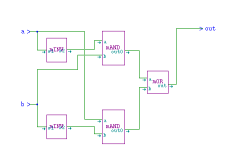
\includegraphics[width=70mm]{exor}
    \caption{Implementazione EXOR}
    \label{ }
    \end{minipage}
    \end{figure}

\\
\\
\textbf{Nota:} le porte AND e OR possono essere realizzate anche implementando le leggi di DeMorgan. Tuttavia, questo tipo di implementazione aumenta leggermente la complessità circuitale, e dunque
si è deciso di optare per la negazione delle porte invertenti, che permette di usare due porte logiche semplici anzichè tre.

\subsection{Elementi di memoria}
Gli elementi di memoria sono circuiti sequenziali che possono avere solo due stati (0 e 1) in grado di passare da uno all'altro sulla base di uno o più segnali di ingresso, e di mantenere lo stato
corrente per un periodo di tempo indefinito.  

\subsubsection{Latch SR}
Il Latch SR (Set-Reset) è un elemento di memoria asincrono dotato di due segnali di ingresso \textbf{\emph{s}} e \textbf{\emph{r}} e di due porte NOR, ciascuna avente un ingresso collegato a 
\emph{s} o \emph{r}, e l'altro collegato all'uscita dell'altra porta NOR.
Il Latch SR ammette un cambiamento di stato sulla sola base dei segnali di ingresso:
\begin{itemize}
    \item Con \emph{s}=1, \emph{r}=0 si passa allo stato di \textbf{SET}: \emph{y}'=0, \emph{y}=1;
    \item Con \emph{s}=0, \emph{r}=1 si passa allo stato di \textbf{RESET}: \emph{y}'=1, \emph{y}=0;
    \item Con \emph{s}=0, \emph{r}=0 lo stato rimane invariato (\textbf{HOLD}).
\end{itemize}
La configurazione \emph{s}=1, \emph{r}=1 non è ammessa. 

\begin{table}[H]
    \begin{minipage}[b]{\textwidth}
    \centering
    \begin{tabular}{|lll|ll|}
        \hline
        \textbf{y'} & \textbf{s} & \textbf{r} & \textbf{f (y)} & \textbf{g (y')} \\ \hline
        0           & 0          & 0          & 1              & 0               \\ 
        0           & 0          & 1          & 0              & 1               \\ 
        0           & 1          & 0          & 1              & 0               \\ 
        0           & 1          & 1          & 0              & 0               \\ 
        1           & 0          & 0          & 0              & 1               \\ 
        1           & 0          & 1          & 0              & 1               \\ 
        1           & 1          & 0          & 1              & 0               \\ 
        1           & 1          & 1          & 0              & 0               \\ \hline
        \end{tabular}
        \caption{Tabella della verità Latch SR}
        \label{tab:my-table}
    \end{minipage}
\end{table}

Il problema legato a questa rete sequenziale, che è asincrona, è la possibilità che si presentino situazioni transitorie che potrebbero modificare le configurazioni degli ingressi in maniera non desiderata o 
non prevedibile. Per risolvere questo problema, è utile introdurre un segnale di sincronismo, come mostrato nei paragrafi che seguono.

\subsubsection{Flip-flop SR}
Nel Flip-flop SR, i due segnali \emph{s} e \emph{r} sono generati da due porte AND, alle quali sono collegati due segnali di ingresso \textbf{\emph{S}} ed \textbf{\emph{R}} 
e un segnale di sincronismo tipicamente denominato \textbf{clock}, di natura generalmente periodica. 
In questo modo, ci si assicura che l'aggiornamento degli stati avvenga solo in momenti ben definiti.
\begin{itemize}
    \item con Clock=1, \emph{S}=1, \emph{R}=0 si ha lo stato di \textbf{set};
    \item con Clock=1, \emph{S}=0, \emph{R}=1 si ha lo stato di \textbf{reset};
    \item con Clock=1, \emph{S}=0, \emph{R}=0 si ha lo stato di \textbf{hold};
    \item con Clock=0, il flip-flop rimane in stato di hold indipendentemente dalla configurazione degli ingressi.
\end{itemize}

\begin{table}[H]
    \begin{minipage}[b]{0.4\textwidth}
    \centering
    \begin{tabular}{|lll|ll|l|}
        \hline
        \textbf{Clk} & \textbf{S} & \textbf{R} & \textbf{s} & \textbf{r} &       \\ \hline
        0            & 0          & 0          & 0          & 0          & HOLD  \\ 
        0            & 0          & 1          & 0          & 0          & HOLD  \\ 
        0            & 1          & 0          & 0          & 0          & HOLD  \\ 
        0            & 1          & 1          & 0          & 0          & HOLD  \\ 
        1            & 0          & 0          & 0          & 0          & HOLD  \\ 
        1            & 0          & 1          & 0          & 1          & RESET \\ 
        1            & 1          & 0          & 1          & 0          & SET   \\ 
        1            & 1          & 1          & 1          & 1          & N.A.  \\ \hline
        \end{tabular}
        \caption{Tabella della verità Flip-flop SR}
        \label{tab:my-table}
    \end{minipage}
    \end{table}
    
    \begin{figure}[ht]
    \begin{minipage}[b]{0.4\textwidth}
    \centering
    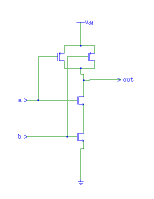
\includegraphics[width=70mm]{nand}
    \caption{Implementazione NAND}
    \label{ }
    \end{minipage}
    \end{figure}

\subsubsection{Flip-flop D-level sensitive}
Il funzionamento di un Flip-flop D-level sensitive è analogo a quello del FFSR, ma ai due segnali \emph{S} e \emph{R} viene sostituito un unico segnale \emph{D}: 
\emph{S} corrisponde a \emph{D}, \emph{R} a \emph{D'}. Questo permette di escludere la configurazione non ammessa \emph{s}=1, \emph{r}=1, 
e di avere durante il periodo di salita del clock due sole configurazioni possibili, ovvero quelle di SET e di RESET. 

\begin{table}[H]
    \begin{minipage}[b]{0.4\textwidth}
    \centering
    \begin{tabular}{|ll|ll|ll|l|}
        \hline
        \textbf{Clk} & \textbf{D} & \textbf{S} & \textbf{R} & \textbf{s} & \textbf{r} &       \\ \hline
        0            & 0          & 0          & 1          & 0          & 0          & HOLD  \\ 
        0            & 1          & 1          & 0          & 0          & 0          & HOLD  \\ 
        1            & 0          & 0          & 1          & 0          & 1          & RESET \\ 
        1            & 1          & 1          & 0          & 1          & 0          & SET   \\ \hline
        \end{tabular}
        \caption{Tabella della verità FF D-level sensitive}
        \label{tab:my-table}
    \end{minipage}
    \end{table}
    
    \begin{figure}[ht]
    \begin{minipage}[b]{0.4\textwidth}
    \centering
    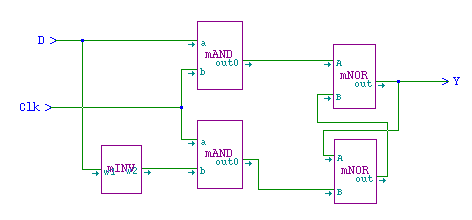
\includegraphics[width=70mm]{ffdls}
    \caption{Implementazione FFDls}
    \label{ }
    \end{minipage}
    \end{figure}


\subsubsection{Flip-flop D-edge triggered}
Il Flip-flop D-edge triggered è un elemento di memoria nel quale l'aggiornamento dello stato è consentito solo sul fronte di salita del clock, a differenza del FFDls che rimane sensibile
alle variazioni degli ingressi per tutta la durata di attività del segnale di clock. E' costruito tramite due FFDls in serie, denominati \textbf{master} e \textbf{slave}
Nel \emph{master} il segnale di clock viene negato, e l'uscita \emph{Y} viene inviata in ingresso allo \emph{slave}. 

\begin{itemize}
    \item Quando Clock=0, il \emph{master} è abilitato a cambiare stato mentre lo \emph{slave} mantiene le uscite stabili;
    \item Quando Clock=1, lo \emph{slave} rileva le variazioni di stato del \emph{master} e le propaga, mentre il \emph{master} è insensibile alle variazioni degli ingressi.
\end{itemize}

La tabella della verità è la medesima del FFDls, in quanto questo Flip-flop è realizzato utilizzando due di questi componenti.

\begin{figure}[H]
    \begin{minipage}[b]{\textwidth}
    \centering
    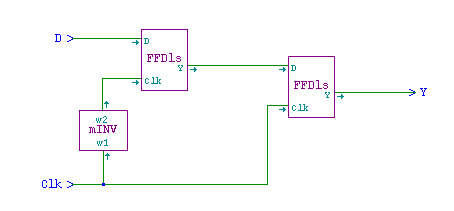
\includegraphics[width=70mm]{ffdet}
    \caption{Implementazione FFDet}
    \label{ }
    \end{minipage}
    \end{figure}

\subsection{Registri}
Un registro è un elemento di memoria in grado di memorizzare vettori di $n$ bit. Ne esistono di differenti tipi, quelli utilizzati in questo progetto sono registri parallelo/parallelo a 4 bit.
Questo tipo di registri è dotato di quattro FFD-edge triggered. Tutti i bit vengono ricevuti in ingresso contemporaneamente, collegando l'ingresso dell'$i$-esimo flip-flop all'$i$-esimo bit del 
vettore in ingresso, e le uscite vengono tutte lette contemporaneamente. 

\begin{figure}[H]
    \begin{minipage}[b]{\textwidth}
    \centering
    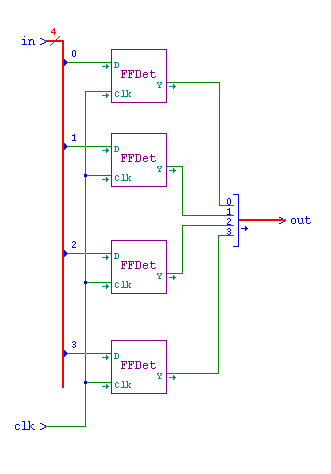
\includegraphics[width=70mm]{reg4}
    \caption{Implementazione registro a 4 bit}
    \label{ }
    \end{minipage}
    \end{figure}

\subsection{Multiplexer}
Il Multiplexer (MUX) è un componente dotato di $x$ ingressi a $n$ bit e di una uscita a $n$ bit, in grado di scegliere il valore che assumerà l'uscita tra quelli in ingresso sulla base di uno o più segnali
di controllo. Il più semplice multiplexer ha 2 ingressi a 1 bit e una uscita a un bit. Funzione, tabella della verità e implementazione sono illustrati di seguito:

$f(a,b,c) = ac' + bc$

\begin{table}[H]
    \begin{minipage}[b]{0.4\textwidth}
    \centering
        \begin{tabular}{|lll|l|}
        \hline
        \textbf{A} & \textbf{B} & \textbf{C} & \textbf{F} \\ \hline
        0          & 0          & 0          & 0          \\ 
        0          & 0          & 1          & 0          \\ 
        0          & 1          & 0          & 0          \\ 
        0          & 1          & 1          & 1          \\ 
        1          & 0          & 0          & 1          \\ 
        1          & 0          & 1          & 0          \\ 
        1          & 1          & 0          & 1          \\ 
        1          & 1          & 1          & 1          \\ \hline
        \end{tabular}
        \caption{Tabella della verità MUX}
        \label{tab:my-table}
    \end{minipage}
    \end{table}
    
    \begin{figure}[H]
    \begin{minipage}[b]{\textwidth}
    \centering
    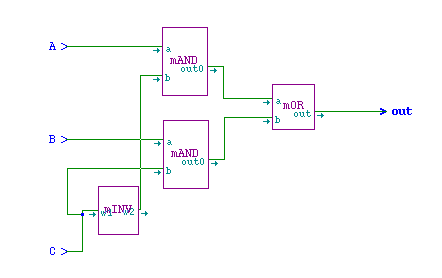
\includegraphics[width=70mm]{mux1}
    \caption{Implementazione MUX}
    \label{ }
    \end{minipage}
    \end{figure}

E' possibile realizzare MUX in grado di scegliere tra due valori a $n$ bit combinando $n$ MUX a 1 bit, ognuno dei quali seleziona
l'$i$-esimo bit del primo o del secondo ingresso a seconda del segnale di controllo. In questo progetto è stato fatto uso di MUX con due ingressi a 4 bit e una uscita a 4 bit. 

\begin{figure}[H]
    \begin{minipage}[b]{\textwidth}
        \centering
        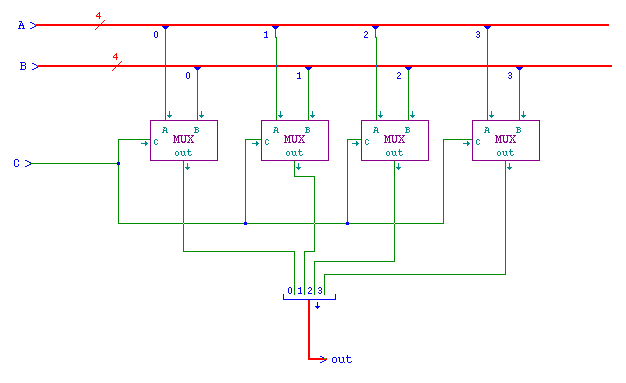
\includegraphics[width=70mm]{mux4}
        \caption{Implementazione MUX a 4 bit}
        \label{ }
    \end{minipage}
\end{figure}

\subsection{Demultiplexer}
Un Demultiplexer (DEMUX) è un componente che funziona in maniera opposta a un MUX: è dotato di un ingresso a $n$ bit e di $x$ uscite a $n$ bit; una di queste uscite assume il valore dell'ingresso,
mentre le altre valgono zero. La selezione è operata sulla base di uno o più segnali di controllo.
Il più semplice DEMUX, illustrato di seguito, è dotato di un ingresso a 1 bit e due uscite a 1 bit.
\\
$f_1 = ac'
f_2 = ac$
\\
\begin{table}[H]
    \begin{minipage}[b]{0.4\textwidth}
    \centering
        \begin{tabular}{|ll|ll|}
        \hline
        \textbf{A} & \textbf{C} & \textbf{F1} & \textbf{F2} \\ \hline
        0          & 0          & 0           & 0           \\ 
        0          & 1          & 0           & 0           \\ 
        1          & 0          & 1           & 0          \\ 
        1          & 1          & 0           & 1           \\ \hline
        \end{tabular}
        \caption{Tabella della verità DEMUX}
        \label{tab:my-table}
    \end{minipage}
    \end{table}
    
    \begin{figure}[H]
    \begin{minipage}[b]{0.4\textwidth}
    \centering
    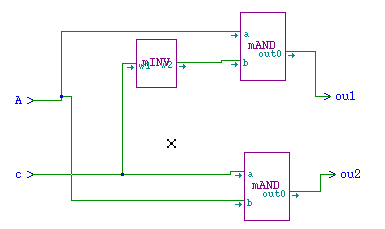
\includegraphics[width=70mm]{demux1}
    \caption{Implementazione DEMUX}
    \label{ }
    \end{minipage}
    \end{figure}

Come per i multiplexer, è possibile implementare un DEMUX con due uscite a $n$ bit combinando $n$ DEMUX a 1 bit, ciascuno dei quali prende in ingresso l'$i$-esimo bit del vettore in ingresso.
Il DEMUX raffigurato di seguito è dotato di un ingresso e due uscite a 4 bit.

\begin{figure}[H]
    \begin{minipage}[b]{0.4\textwidth}
        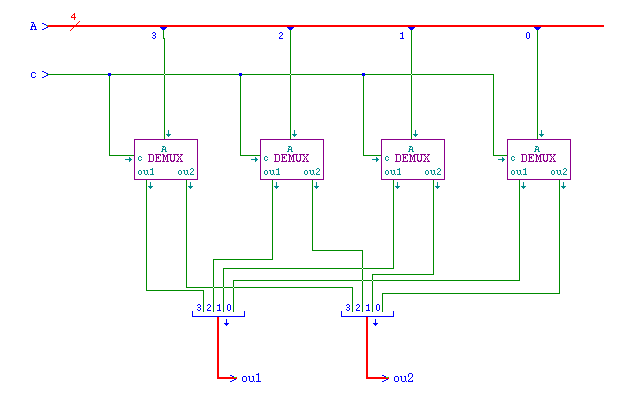
\includegraphics[width=70mm]{demux4}
        \caption{Implementazione DEMUX a 4 bit}
        \label{ }
    \end{minipage}
\end{figure}

\subsection{Macro aritmetiche}
\subsubsection{Half adder}
Un Half Adder (HA) è una rete combinatoria in grado di calcolare la somma di due bit. E' dotato di due ingressi a un bit (gli addendi) e di due uscite S e Cout che rappresentano Il
risultato della somma e il riporto in uscita, rispettivamente.
Le equazioni corrispondenti alle due uscite sono:
$S = A \oplus Cin$
$Cout = ACin$

\begin{table}[H]
    \begin{minipage}[b]{0.4\textwidth}
    \centering
    \begin{tabular}{|l|l|l|l|}
        \hline
        \textbf{A} & \textbf{Cin} & \textbf{S} & \textbf{Cout} \\ \hline
        0          & 0            & 0          & 0             \\ 
        0          & 1            & 1          & 0             \\ 
        1          & 0            & 1          & 0             \\ 
        1          & 1            & 0          & 1             \\ \hline
        \end{tabular}
        \caption{Tabella della verità HA}
        \label{table:student}
    \end{minipage}
    \end{table}
    
    \begin{figure}[H]
    \begin{minipage}[b]{0.4\textwidth}
    \centering
    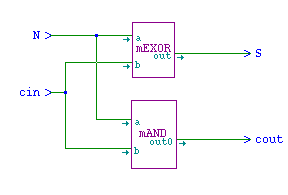
\includegraphics[width=70mm]{ha}
    \caption{Implementazione HA}
    \label{ }
    \end{minipage}
    \end{figure}

\subsubsection{Full adder}
Un Full Adder (FA) è una rete combinatoria che calcola la somma di tre bit. E' dotato di tre ingressi A, B e Cin che rappresentano il primo addendo, il seccondo addendo e il riporto
in ingresso, e di due uscite S e Cout che rappresentano il risultato della somma e il riporto in uscita, rispettivamente. 
Le equazioni delle due uscite sono:
$$
S = Cin \oplus (A \oplus B)
cout = AB + Cin(A + B)
$$
E' possibile implementare questo componente utilizzando due HA in cascata e una porta NOT. Il primo HA calcola la somma dei due addendi, e al risultato viene sommato il riporto in ingresso
tramite il secondo HA.
Il riporto in uscita del FA corrisponde alla disgiunzione logica dei riporti in uscita dei due HA.

\begin{table}[H]
    \begin{minipage}[b]{0.4\textwidth}
    \centering
    \begin{tabular}{|l|l|l|l|l|}
        \hline
        \textbf{A} & \textbf{B} & \textbf{Cin} & \textbf{S} & \textbf{Cout} \\ \hline
        0          & 0          & 0            & 0          & 0             \\ 
        0          & 0          & 1            & 1          & 0             \\ 
        0          & 1          & 0            & 1          & 0             \\ 
        0          & 1          & 1            & 0          & 1             \\ 
        1          & 0          & 0            & 1          & 0             \\ 
        1          & 0          & 1            & 0          & 1             \\ 
        1          & 1          & 0            & 0          & 1             \\ 
        1          & 1          & 1            & 1          & 1             \\ \hline
        \end{tabular}
        \caption{Tabella della verità FA}
        \label{table:student}
    \end{minipage}
    \end{table}
    
    \begin{figure}[H]
    \begin{minipage}[b]{0.4\textwidth}
    \centering
    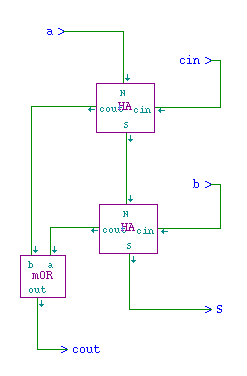
\includegraphics[width=70mm]{FA}
    \caption{Implementazione FA}
    \label{ }
    \end{minipage}
    \end{figure}

\subsubsection{Complementatore}
Per trasformare un numero intero nel rispettivo complemento a 2, è sufficiente complementare i singoli bit che lo compongono, e poi sommare 1 al vettore di bit così ottenut0.
Per realizzare un circuito in grado di calcolare il complemento a due di un numero si è dunque iniziato collegando ciascun bit del valore in ingresso ad un inverter, per poi sommare
i singoli bit tramite half adder, collegando il riporto in ingresso del primo HA alla differenza di potenziale e il riporto in uscita all'HA successivo.

\begin{figure}[H]
    \begin{minipage}[c]{\textwidth}
    \centering    
    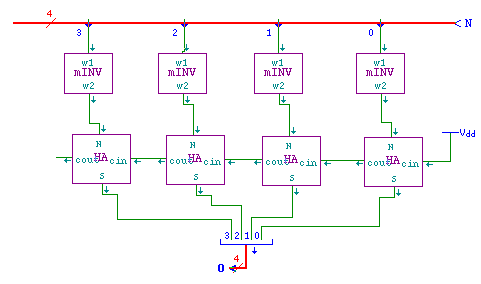
\includegraphics[width=70mm]{complementoadue}
    \caption{Implementazione Complementatore}
    \label{ }
    \end{minipage}
\end{figure}


\subsubsection{RCA a 4bit}
Un Ripple Carry Adder (RCA) è una macro funzionale per l'addizione di valori a $n$bit. Il suo funzionamento si basa sullo schema classico dell'addizione in colonna: il primo bit
dell'operando A viene sommato al primo bit dell'operando B, il bit di somma viene aggiunto al vettore di bit dell'uscita mentre il riporto in uscita viene aggiunto alla somma dei due bit successivi.
Questo schema viene implementato tramite FA in serie, dove il riporto in ingresso corrisponde al riporto in uscita del FA precedente, con l'eccezione del primo FA, il cui riporto in ingresso è
collegato alla massa.

\begin{figure}[H]
    \begin{minipage}[c]{\textwidth} 
    \centering   
    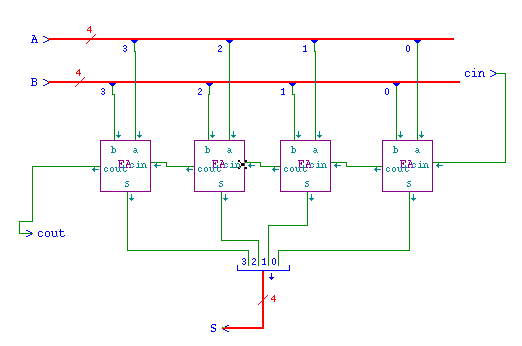
\includegraphics[width=70mm]{RCA}
    \caption{Implementazione RCA}
    \label{ }
    \end{minipage}
\end{figure}

\subsubsection{MAC}
Un MAC (acronimo di multiply-and-accumulate) è un componente base utilizzato per la realizzazione di moltiplicatori. Questo componente calcola il prodotto tra due bit (corrispondente al prodotto logico)
e la somma tra i due bit in ingresso. E' dotato di tre ingressi A, B e Cin e di quattro uscite S, Cout, Aout, Bout. Le prime due uscite rappresentano il bit di somma e il riporto in uscita,
che vengono propagati al MAC sottostante (S) e a quello adiacente (Cout); mentre Aout e Bout propagano i bit in ingresso al MAC successivo lungo la diagonale (Aout) e a quello adiacente (Bout).
\begin{figure}[H]
    \centering
    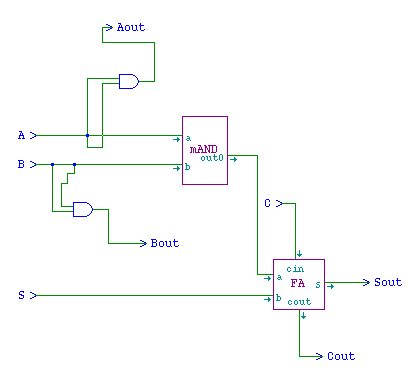
\includegraphics[width=0.4\textwidth]{MAC}
\end{figure}

\begin{table}[H]
    \centering
    \begin{tabular}{|cccc|cccc|}
    \hline
    \textbf{A} & \textbf{B} & \textbf{Cin} & \textbf{Sin} & \textbf{Sout} & \textbf{Cout} & \textbf{Aout} & \textbf{Bout} \\ \hline
    0          & 0          & 0            & 0            & 0             & 0             & 0             & 0             \\ 
    0          & 0          & 0            & 1            & 1             & 0             & 0             & 0             \\ 
    0          & 0          & 1            & 0            & 1             & 0             & 0             & 0             \\ 
    0          & 0          & 1            & 1            & 0             & 1             & 0             & 0             \\ 
    0          & 1          & 0            & 0            & 0             & 0             & 0             & 1             \\ 
    0          & 1          & 0            & 1            & 1             & 0             & 0             & 1             \\ 
    0          & 1          & 1            & 0            & 1             & 0             & 0             & 1             \\ 
    0          & 1          & 1            & 1            & 0             & 1             & 0             & 1             \\ 
    1          & 0          & 0            & 0            & 0             & 0             & 1             & 0             \\ 
    1          & 0          & 0            & 1            & 1             & 0             & 1             & 0             \\ 
    1          & 0          & 1            & 0            & 1             & 0             & 1             & 0             \\ 
    1          & 0          & 1            & 1            & 0             & 1             & 1             & 0             \\ 
    1          & 1          & 0            & 0            & 1             & 0             & 1             & 1             \\ 
    1          & 1          & 0            & 1            & 0             & 1             & 1             & 1             \\ 
    1          & 1          & 1            & 0            & 0             & 1             & 1             & 1             \\ 
    1          & 1          & 1            & 1            & 1             & 1             & 1             & 1             \\ \hline
    \end{tabular}
    \caption{Tabella della verità MAC}
    \label{tab:my-table}
    \end{table}

\subsubsection{Moltiplicatore a 4 bit}
Il moltiplicatore a 4 bit utilizzato in questo progetto è stato utilizzato collegando i componenti illustrati in precedenza, andando a formare una struttura a matrice.
La struttura conta quattro file di MAC. In ogni fila, il primo componente è collegato al $i$-esimo bit del secondo operando (B).
Nella prima fila, ogni MAC é collegato a uno dei bit del primo operando (A), che viene propagato al MAC sulla riga sottostande in direzione diagonale.
Il bit di somma viene propagato verso il basso, entrando in uno dei MAC sottostanti o nel vettore di bit in uscita, mentre il riporto in uscita si propaga orizzontalmente, analogamente a ciò che accade
nel ripple-carry adder.
Questo schema ricalca lo schema della moltiplicazione in colonna, ma anzichè ottenere 4 prodotti parziali, che vanno poi sommati tra loro, l'addizione tra il prodotto di due bit e il prodotto dei due
bit superiori viene effettuato contestualmente alla moltiplicazione, in modo da produrre immediatamente il bit del prodotto finale.

\begin{figure}[H]
    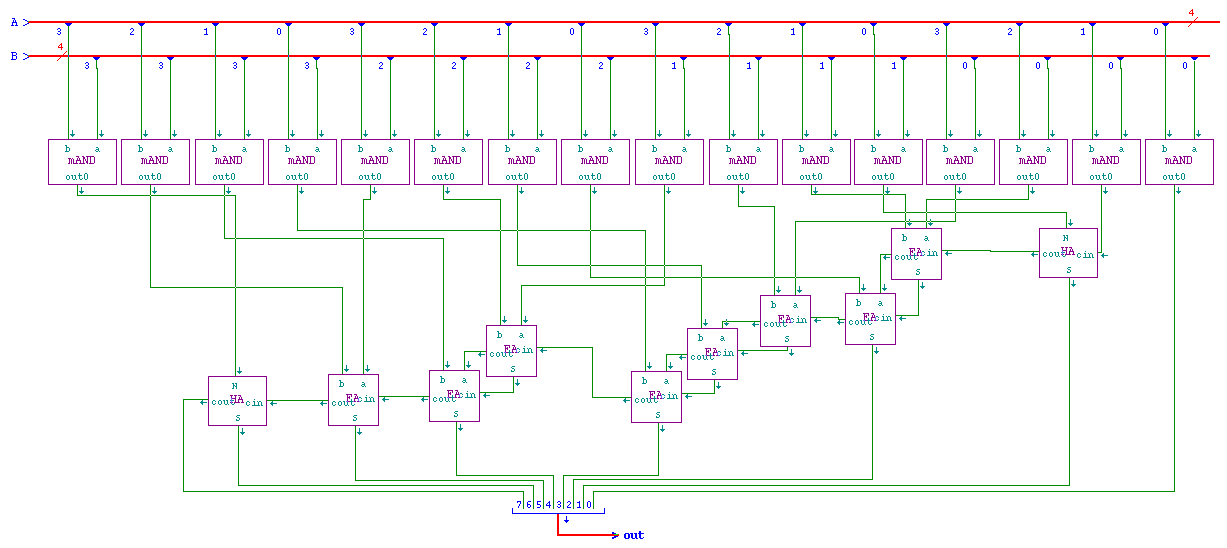
\includegraphics[width=0.8\textwidth]{MUL}
    \centering
\end{figure}


\section{Data Path}
\begin{figure}[H]
    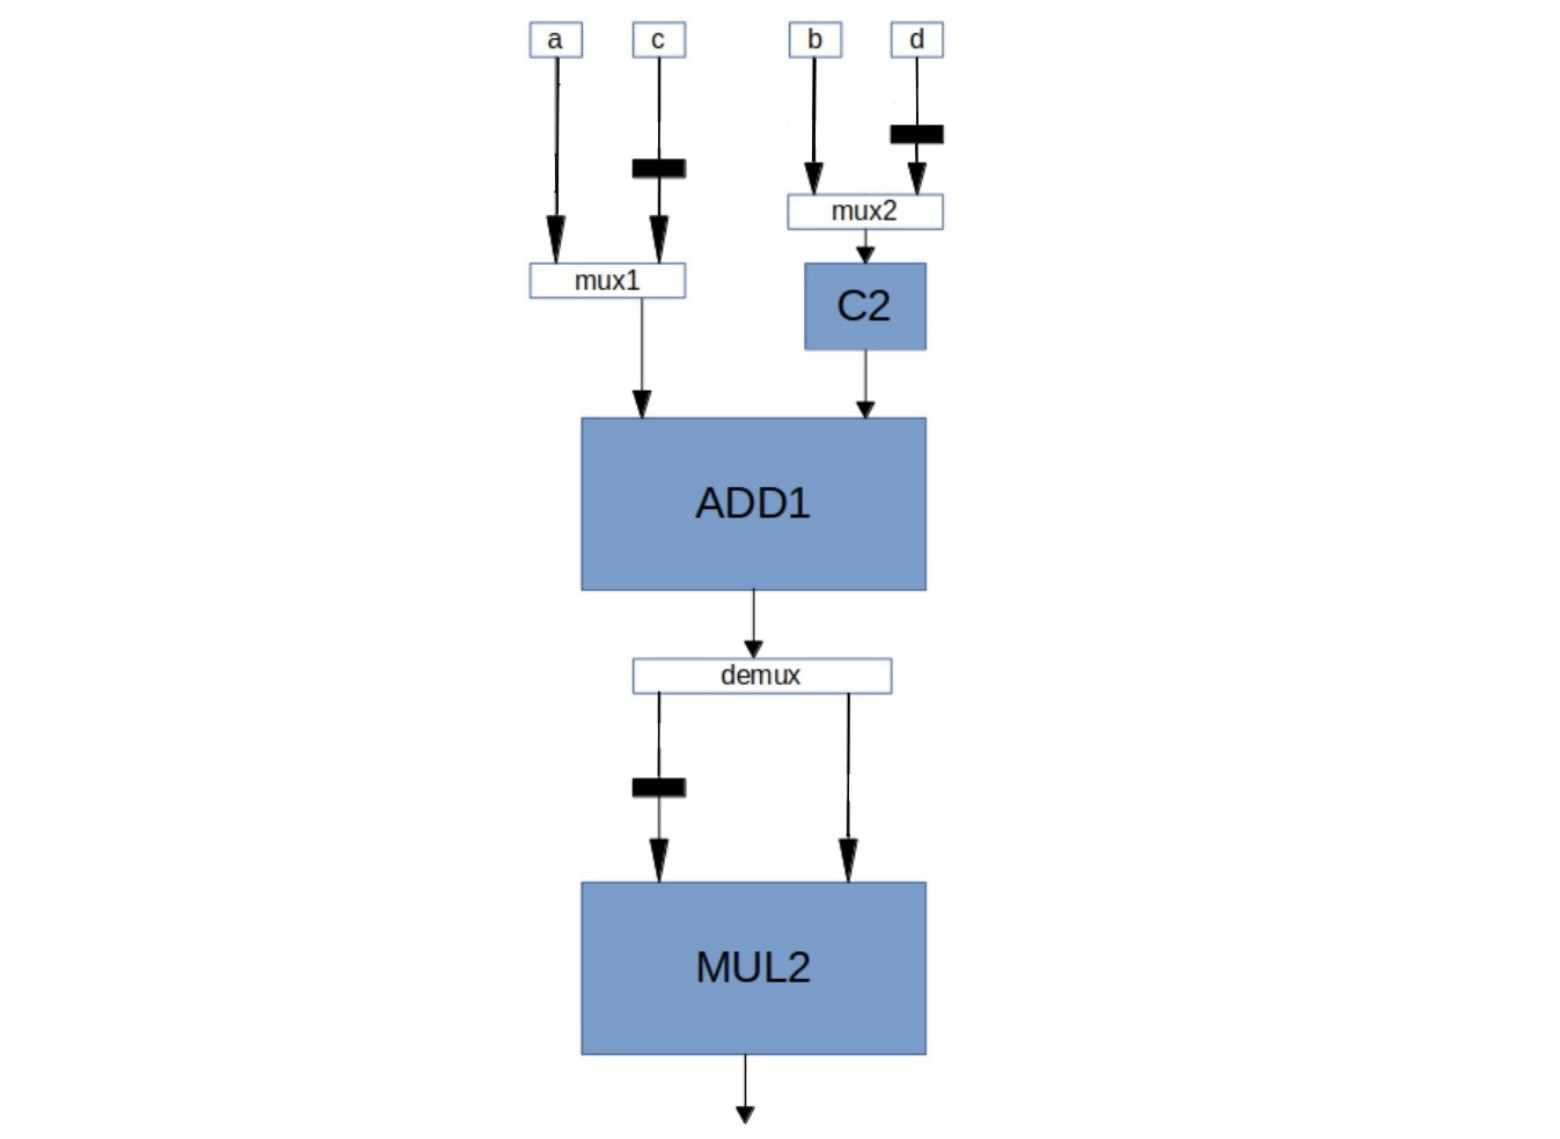
\includegraphics[width=0.7\textwidth]{datapath}
    \centering
\end{figure}


\section{Control Unit}

\subsection{Specifica}
Il circuito che si sta progettando necessita di due multiplexer e un demultiplexer, tutti con un singolo segnale di controllo; e di due cicli di clock.
Durante il primo ciclo di clock, tutti e tre i componenti devono selezionare l'ingresso/uscita di sinistra (segnale 0), mentre nel secondo ciclo di clock viene selezionato l'ingresso/uscita
di destra (segnale 1).
Dal momento che per tutti e tre i componenti controllati dalla CU il segnale assume lo stesso valore all'interno del medesimo ciclo di clock, è possibile utilizzare un unico segnale
di controllo (denominato C).

\begin{table}[H]
    \begin{minipage}[c]{\textwidth}
    \centering
    \begin{tabular}{|c|ccc|c|}
        \hline
        \textbf{Ciclo di Clock} & \textbf{MUX1} & \textbf{MUX2} & \textbf{DEMUX} & \textbf{C}\\ \hline
        0                       & 0             & 0             & 0              & 0         \\ 
        1                       & 1             & 1             & 1              & 1         \\ \hline
        \end{tabular}
    \end{minipage}
    \end{table}

E' possibile implementare questa specifica tramite una macchina a stati finiti che può assumere due stati (Ciclo 0 e Ciclo 1) e produce un unico segnale in uscita. 
La funzione di uscita dipende unicamente dallo stato presente, mentre la funzione di stato futuro dipende dallo stato presente e dagli ingressi: si tratta dunque di una macchina di Moore.

\begin{figure}[H]
    \centering
    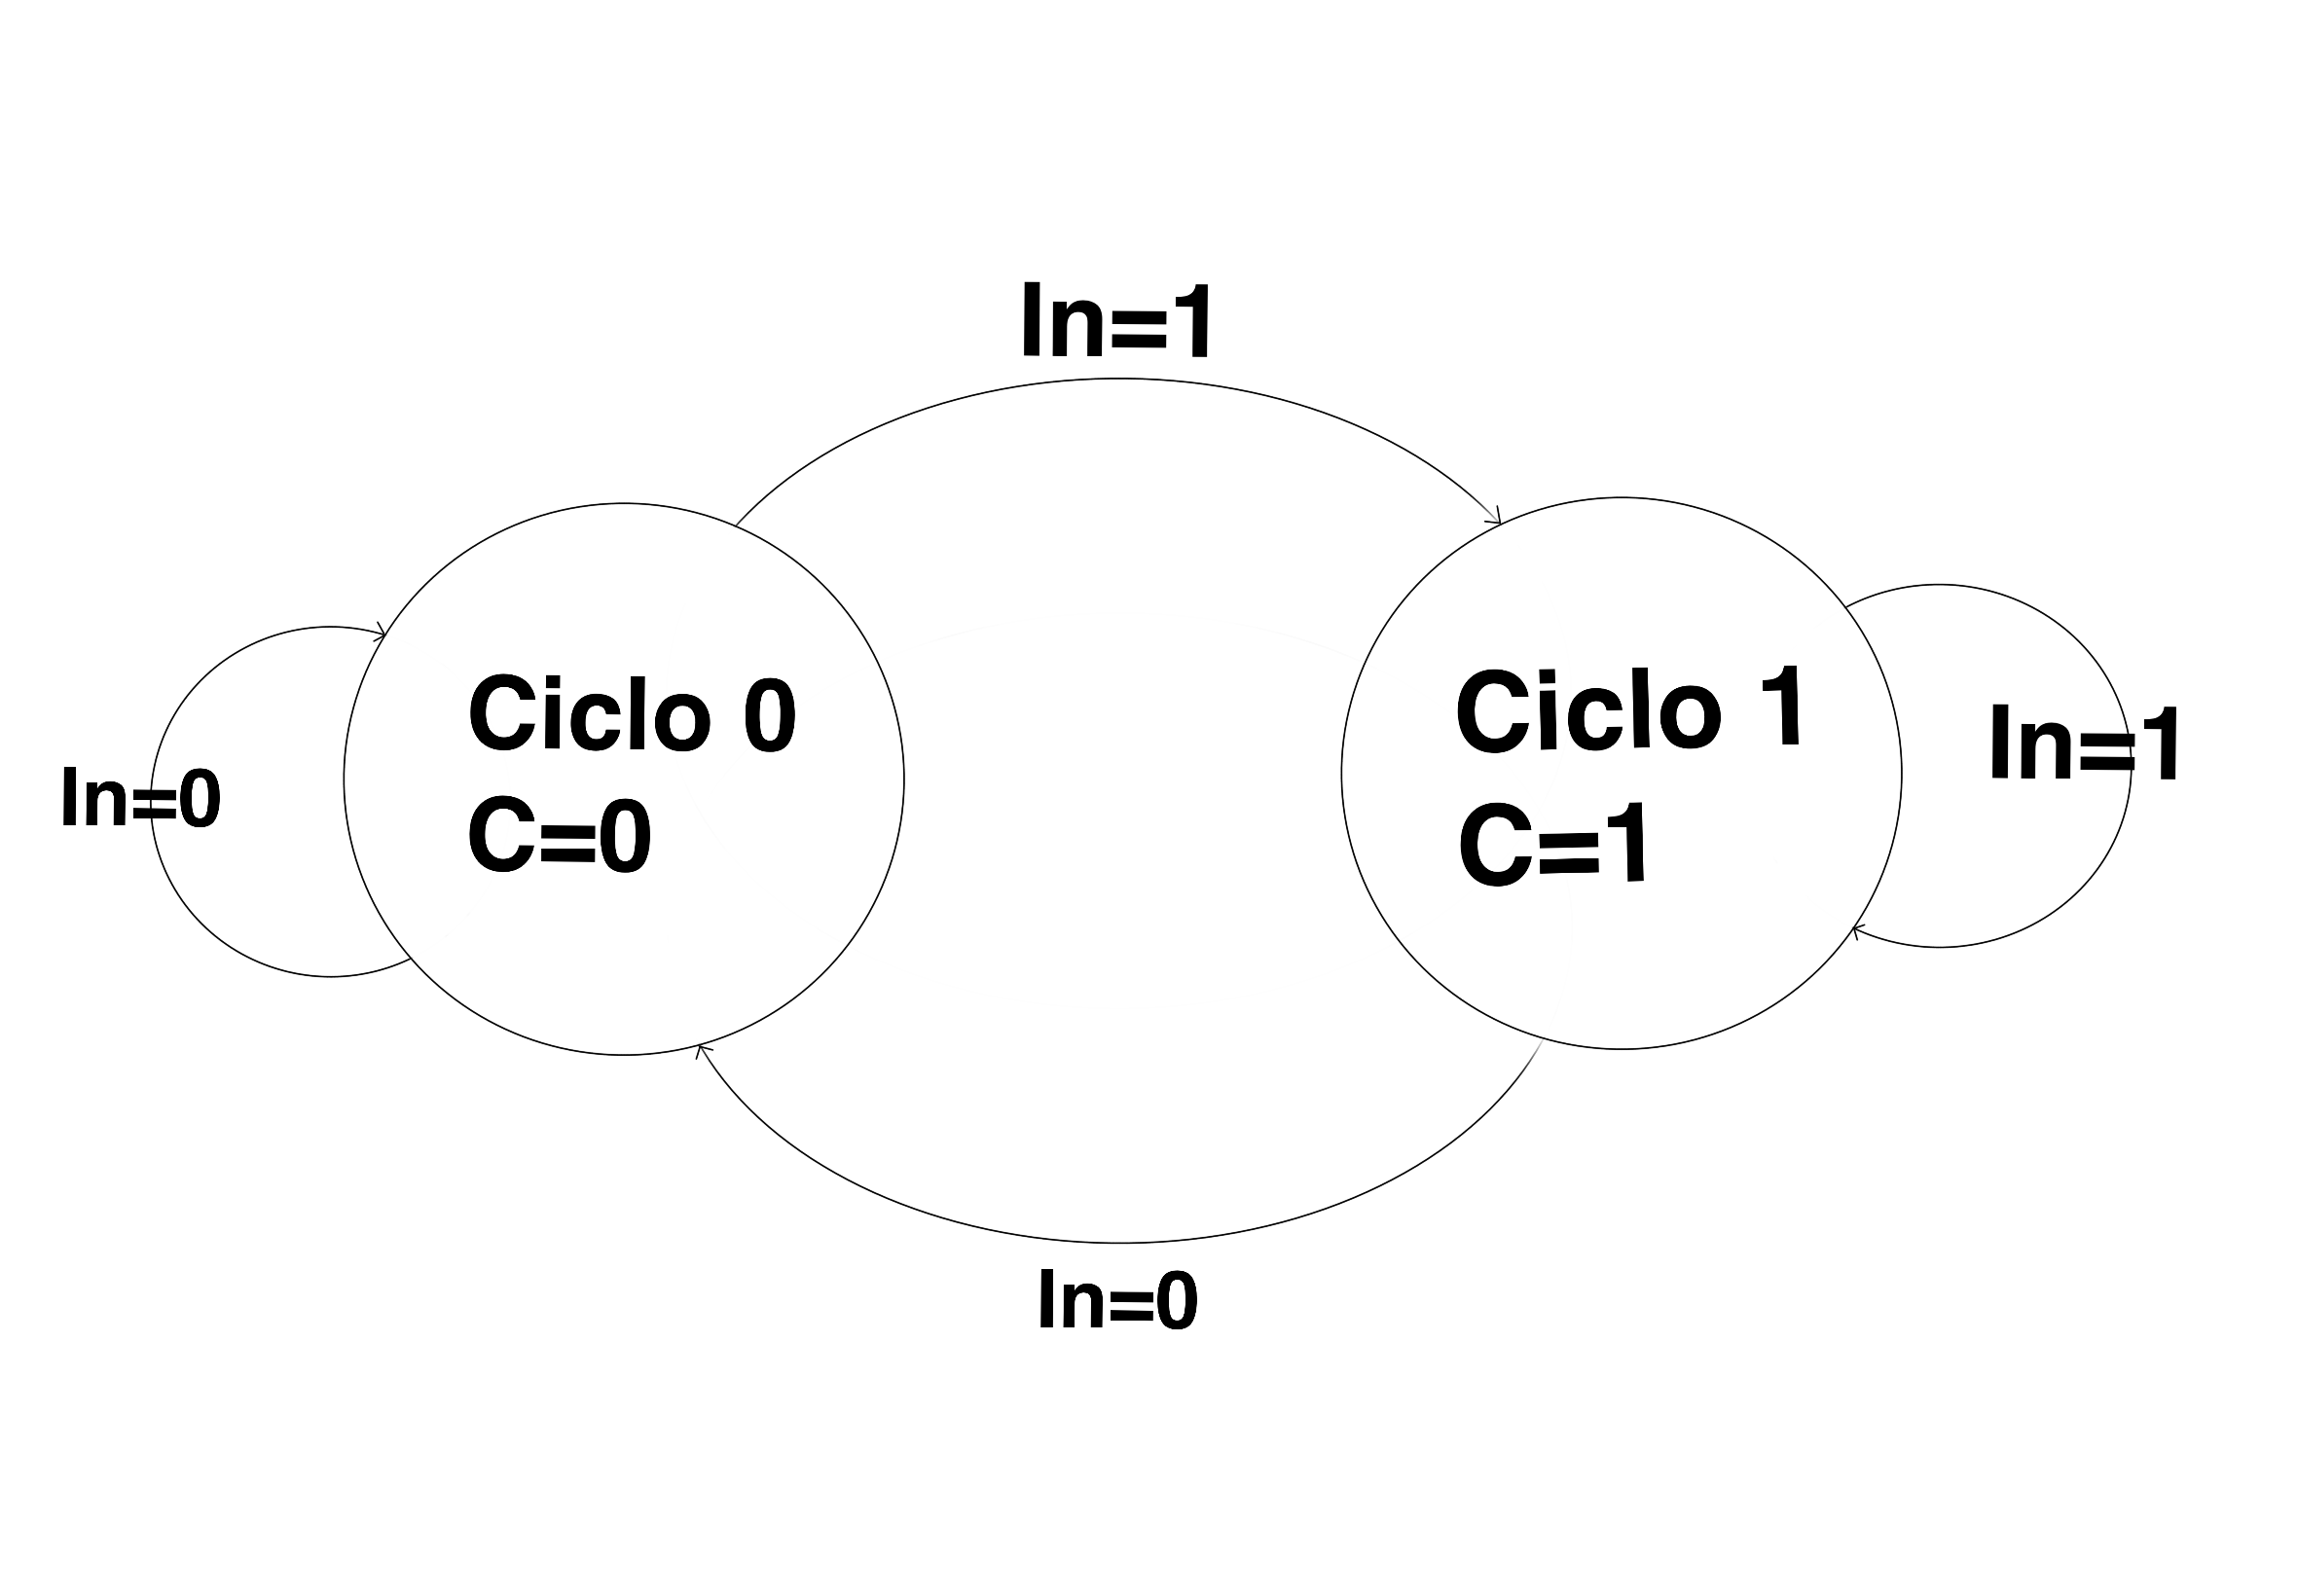
\includegraphics[width=0.7\textwidth]{statediag}
\end{figure}

I due stati della macchina di Moore possono essere codificati con un singolo bit S.

\begin{table}[H]
    \begin{minipage}[c]{\textwidth}
    \centering
    \begin{tabular}{|c|c|c|}
        \hline
        \textbf{S} & \textbf{C} & \textbf{Sn} \\ \hline
        0          & 0          & 1           \\ 
        1          & 1          & 0           \\ \hline
        \end{tabular}
        \caption{Codifica degli stati}
        \label{tab:my-table}
    \end{minipage}
    \end{table}

Le funzioni di uscita e stato futuro risultano essere:\\
\textbf{Sn = S'}\\
\textbf{C = S}\\

\subsection{Implementazione della macchina di Moore}
Per poter implementare la control unit tramite macchina di Moore, è necessario introdurre un segnale in ingresso, che imposti lo stato iniziale a 0 e permetta il cambiamento
di stato. 
\begin{table}[H]
    \begin{minipage}[c]{\textwidth}
    \centering
    \begin{tabular}{|c|c|c|c|}
        \hline
        \textbf{In} &\textbf{S}  & \textbf{C} & \textbf{Sn} \\ \hline
        0           &0           & 0          & 0           \\
        0           &1           & 0          & 0           \\
        1           &0           & 1          & 1           \\ 
        1           &1           & 1          & 0           \\ \hline
        \end{tabular}
    \end{minipage}
    \end{table}

Le funzioni di uscita e stato futuro risultano dunque essere:
\\
\textbf{Sn = InS'}\\ 
\textbf{C = In'S + InS = S}
\\
\\
Lo stato presente viene conservato tramite un FFD-edge triggered,
che viene aggiornato solo sul fronte di salita del clock (che in questo caso è rappresentato da un interrutore manovrato manualmente). 
L'uscita del FF viene portata ai componenti che necessitano del segnale di controllo e all'interno di un inverter collegato all'ingresso di una porta AND, il cui segnale viene portato
all'interno del FF. L'altro ingresso della porta AND è collegato a un interruttore, inizialmente impostato su 0, rappresentante il segnale di ingresso. 
\\
\\
\begin{figure}[ht]
    \begin{minipage}[c]{\textwidth}
    \centering
    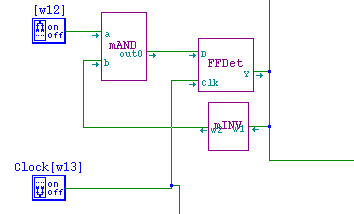
\includegraphics[width=70mm]{cu}
    \caption{Implementazione Control Unit}
    \label{ }
    \end{minipage}
\end{figure}

\newpage

\section{Simulazione e analisi del progetto}
\subsection{Verifica funzionale}
In questa sezione sono riportate delle immagini illustrative di alcune simulazioni effettuate per testare la funzionalità del circuito. In tutto sono riportate tre simulazioni, per ciascuna vengono 
illustrati entrambi i cicli di clock.

\begin{figure}[H]
    \begin{minipage}[c]{\textwidth}
    \centering    
    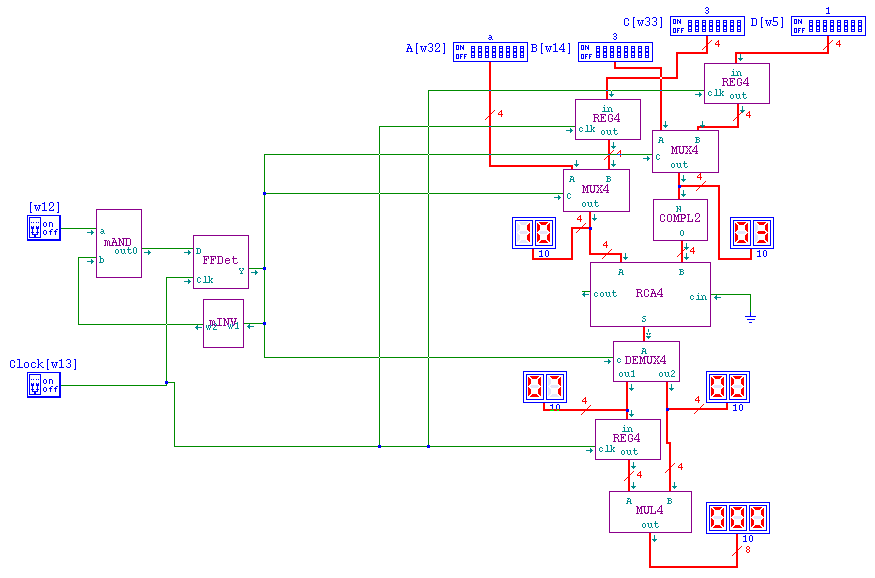
\includegraphics[width=100mm]{s1c0}
    \caption{Simulazione 1: clock 0}
    \label{ }
    \end{minipage}
\end{figure}

\begin{figure}[H]
    \begin{minipage}[c]{\textwidth}
    \centering
    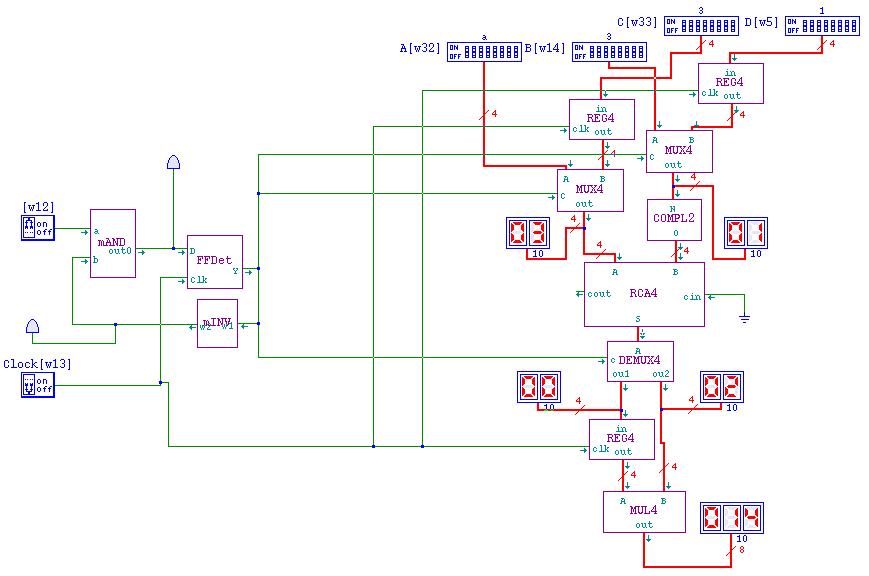
\includegraphics[width=100mm]{s1c1}
    \caption{Simulazione 1: ciclo di clock 1}
    \label{ }
    \end{minipage}
\end{figure}

\begin{figure}[H]
    \begin{minipage}[c]{\textwidth}
    \centering
    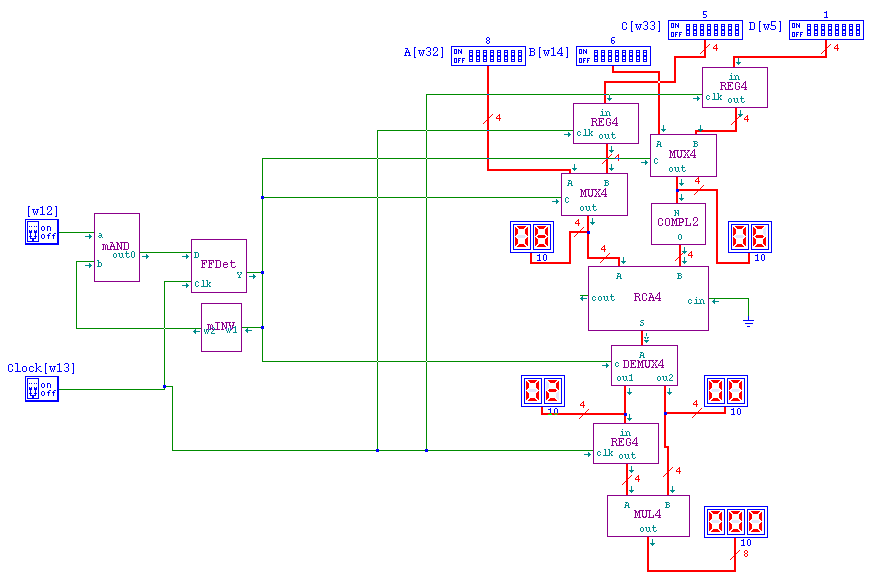
\includegraphics[width=100mm]{s2c0}
    \caption{Simulazione 2: ciclo di clock 0}
    \label{ }
    \end{minipage}
\end{figure}

\begin{figure}[H]
    \begin{minipage}[c]{\textwidth}
    \centering
    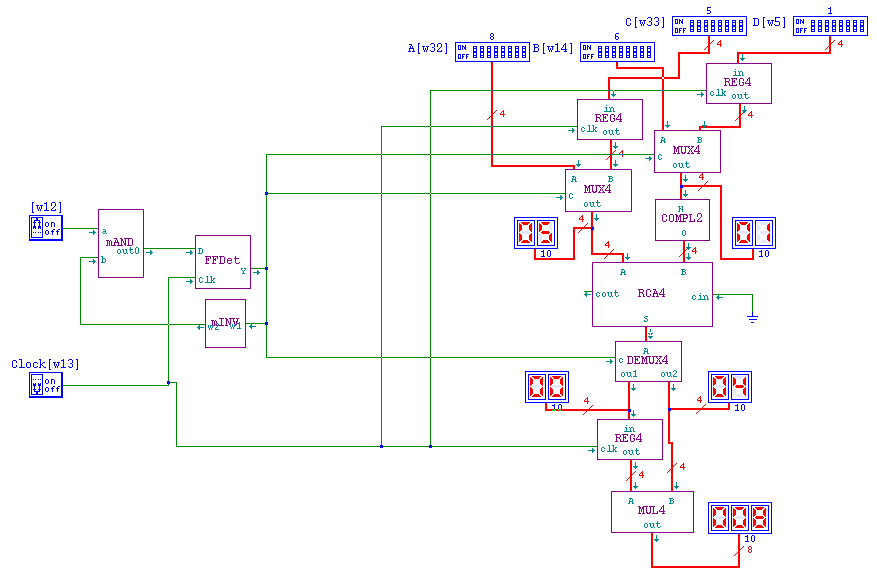
\includegraphics[width=100mm]{s2c1}
    \caption{Simulazione 2: ciclo di clock 1}
    \label{ }
    \end{minipage}
\end{figure}

\begin{figure}[H]
    \begin{minipage}[c]{\textwidth}
    \centering
    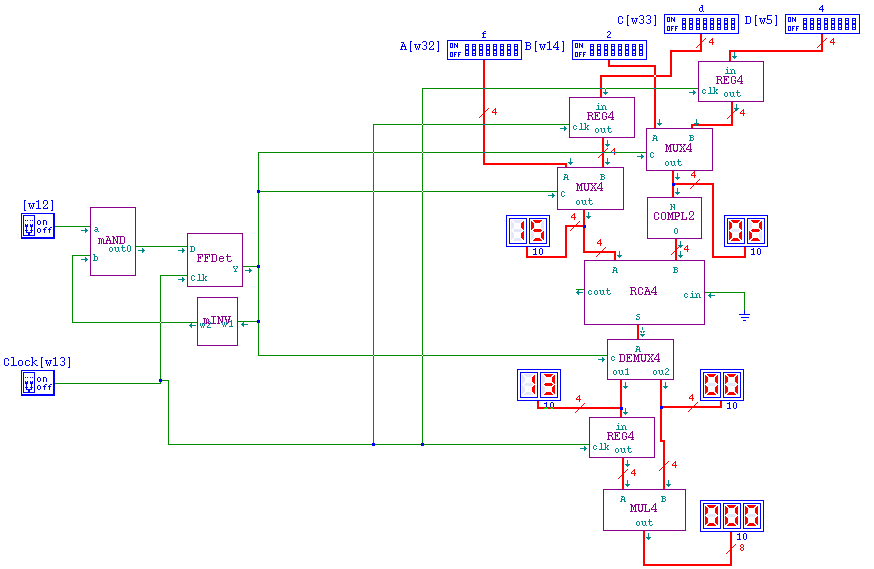
\includegraphics[width=100mm]{s3c0}
    \caption{Simulazione 3: ciclo di clock 0}
    \label{ }
    \end{minipage}
\end{figure}

\begin{figure}[H]
    \begin{minipage}[c]{\textwidth}
    \centering
    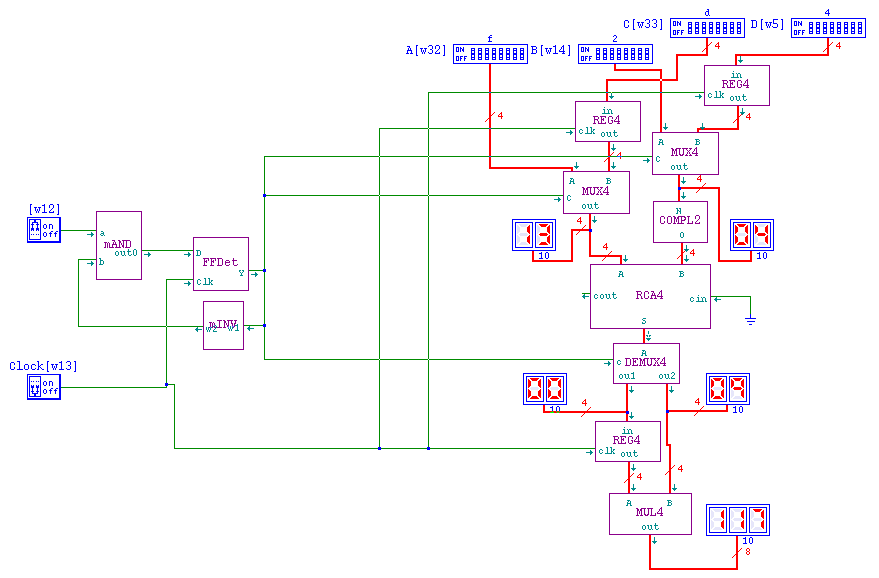
\includegraphics[width=100mm]{s3c1}
    \caption{Simulazione 3: ciclo di clock 1}
    \label{ }
    \end{minipage}
\end{figure}

\subsection{Valutazione di prestazioni e complessità}

\begin{table}[H]
    \begin{minipage}[c]{\textwidth}
    \centering
    \begin{tabular}{|c|c|c|c|c|c|c|}
    \hline
                  & \textbf{NOT} & \textbf{NAND} & \textbf{NOR} & \textbf{AND} & \textbf{OR} & \textbf{EXOR} \\ \hline
    \textbf{Area} & 1            & 1             & 1            & 2            & 2           & 5             \\ 
    \textbf{Tp}   & 1            & 1             & 1            & 2            & 2           & 3             \\ 
    \textbf{Tc}   & 1            & 1             & 1            & 2            & 2           & 2             \\ \hline
    \end{tabular}
    \caption{Area e prestazioni porte logiche}
    \label{tab:my-table}
\end{minipage}
\end{table}

\begin{table}[H]
    \begin{minipage}[c]{\textwidth}
    \centering
    \begin{tabular}{|c|c|c|c|c|c|c|}
    \hline
                  & \textbf{Latch SR} & \textbf{FFSR}          & \textbf{FFDls}      & \textbf{FFDet}           & \textbf{Registri} \\ \hline
    \textbf{Area} & 2*A(NOR)=2        & A(LSR)+2*A(AND)=6      & A(FFSR)+A(NOT)=5    & 2*A(FFDls)+A(NOT)=11     & 4*A(FFDet)=44     \\ 
    \textbf{Tp}   & 2*Tp(NOR)=2       & Tp(LSR)+2*Tp(AND)=6    & Tp(FFSR)+Tp(NOT)=7  & 2*Tp(FFDls)+Tp(NOT)=15   & 4*Tp(FFDet)=60    \\ 
    \textbf{Tc}   & Tc(NOR)=1         & Tc(LSR)+Tc(AND)=3      & Tc(FFSR)=3          & 2*Tc(FFDls)=6            & Tc(FFDet)=6       \\ \hline
    \end{tabular}
    \caption{Area e prestazioni elementi di memoria}
    \label{tab:my-table}
\end{minipage}
\end{table}

\begin{table}[H]
    \begin{minipage}[c]{\textwidth}
    \centering
        \begin{tabular}{|c|c|c|c|c|c|c|}
        \hline
                      & \textbf{MUX}               & \textbf{MUX 4 BIT} & \textbf{DEMUX}     & \textbf{DEMUX 4 BIT} \\ \hline
        \textbf{Area} & 2*A(AND)+A(OR)+A(NOT) = 7  & 4*A(MUX) = 24      & 2*A(AND)+A(INV)=5  & 4*A(DEMUX)=20        \\ 
        \textbf{Tp}   & Tp(NOT)+Tp(AND)+Tp(OR) = 5 & 4*Tp(MUX) = 20     & Tp(NOT)+Tp(AND)=3  & 4*Tp(DEMUX)=12       \\ 
        \textbf{Tc}   & Tc(AND)+Tc(OR) = 4         & Tc(MUX) = 4        & Tc(AND)=2          & Tc(DEMUX)=2          \\ \hline
        \end{tabular}
        \caption{Area e prestazioni componenti di selezione}
        \label{tab:my-table}
    \end{minipage}
\end{table}

\begin{table}[H]
    \begin{minipage}[c]{\textwidth}
    \centering
    \begin{tabular}{|c|c|c|c|c|c|c|}
    \hline
                  & \textbf{HA}              & \textbf{FA}      & \textbf{C2}            & \textbf{RCA4}  & \textbf{MAC}      & \textbf{MUL4}  \\ \hline
    \textbf{Area} & A(AND)+A(EXOR)=7         & 2*A(HA)+A(OR)=9  & 4*A(HA)+4*A(NOT)=32    & 4*A(FA)=45     & A(AND)+A(FA)=11   & 1*A(MAC)=176   \\ 
    \textbf{Tp}   & Tp(AND)+Tp(EXOR)=5       & Tp(HA)+Tp(OR)=7  & 4*Tp(HA)+4*Tp(NOT)=24  & 4*Tp(FA)=96    & Tp(AND)+Tp(FA)=9  & 16*Tp(MAC)=144 \\ 
    \textbf{Tc}   & min(Tc(AND),Tc(EXOR))=2  & Tc(HA)=2         & Tc(HA)+Tc(NOT)=3       & Tc(FA)=2       & Tc(AND)=2         & Tc(MAC)=2      \\ 
    \textbf{Rate} & 1/Tp(HA)                 & 1/Tp(FA)         & 1/Tp(C2)               & 1/Tp(RCA)      & 1/Tp(MAC)         & 1/Tp(MUL)      \\ \hline
    \end{tabular}
    \caption{Area e prestazioni macro artimetiche}
    \label{tab:my-table}
\end{minipage}
\end{table}

\subsection{Stima di complessità circuitale e prestazioni}
Effettuare la stima per ogni componente combinatorio (tempo di propagazione con modello di ritardo unitario), per ogni stadio 
(tempo di propagazione) e per l’intero progetto (latenza)
Determinare la durata minima del periodo di clock a cui può funzionare il circuito
Dipendenza di prestazioni e complessità dal numero di bit degli operandi

TClock > Tp(RCA4) +Tp(C2) + Tp(MUL)

\end{document}